\documentclass{beamer}

\mode<presentation>
{
  \usetheme{default}
  \usecolortheme{default}
  \usefonttheme{default}
  \setbeamertemplate{navigation symbols}{}
  \setbeamertemplate{caption}[numbered]
  \setbeamertemplate{footline}[page number]
  \setbeamercolor{frametitle}{fg=white}
  \setbeamercolor{footline}{fg=black}
} 

\usepackage[english]{babel}
\usepackage[utf8x]{inputenc}
\usepackage{tikz}
\usepackage{listings}
\usepackage{courier}
\usepackage{array}
\usepackage{bold-extra}
\usepackage{minted}
\usepackage{fancyvrb}

\xdefinecolor{darkblue}{rgb}{0.1,0.1,0.7}
\xdefinecolor{darkgreen}{rgb}{0,0.5,0}
\xdefinecolor{darkgrey}{rgb}{0.35,0.35,0.35}
\xdefinecolor{darkorange}{rgb}{0.8,0.5,0}
\xdefinecolor{darkred}{rgb}{0.7,0,0}
\xdefinecolor{dianablue}{rgb}{0.18,0.24,0.31}
\definecolor{commentgreen}{rgb}{0,0.6,0}
\definecolor{stringmauve}{rgb}{0.58,0,0.82}

\lstset{ %
  backgroundcolor=\color{white},      % choose the background color
  basicstyle=\ttfamily\small,         % size of fonts used for the code
  breaklines=true,                    % automatic line breaking only at whitespace
  captionpos=b,                       % sets the caption-position to bottom
  commentstyle=\color{commentgreen},  % comment style
  escapeinside={\%*}{*)},             % if you want to add LaTeX within your code
  keywordstyle=\color{blue},          % keyword style
  stringstyle=\color{stringmauve},    % string literal style
  showstringspaces=false,
  showlines=true
}

\lstdefinelanguage{scala}{
  morekeywords={abstract,case,catch,class,def,%
    do,else,extends,false,final,finally,%
    for,if,implicit,import,match,mixin,%
    new,null,object,override,package,%
    private,protected,requires,return,sealed,%
    super,this,throw,trait,true,try,%
    type,val,var,while,with,yield},
  otherkeywords={=>,<-,<\%,<:,>:,\#,@},
  sensitive=true,
  morecomment=[l]{//},
  morecomment=[n]{/*}{*/},
  morestring=[b]",
  morestring=[b]',
  morestring=[b]"""
}

\title[2017-06-02-odg-shredtypes]{Portable Rich Data Representation}
\author{Jim Pivarski}
\institute{Princeton University -- DIANA}
\date{June 5, 2017}

\begin{document}

\logo{\pgfputat{\pgfxy(0.11, 8)}{\pgfbox[right,base]{\tikz{\filldraw[fill=dianablue, draw=none] (0 cm, 0 cm) rectangle (50 cm, 1 cm);}}}\pgfputat{\pgfxy(0.11, -0.6)}{\pgfbox[right,base]{\tikz{\filldraw[fill=dianablue, draw=none] (0 cm, 0 cm) rectangle (50 cm, 1 cm);}\includegraphics[height=0.99 cm]{diana-hep-logo.png}\tikz{\filldraw[fill=dianablue, draw=none] (0 cm, 0 cm) rectangle (4.9 cm, 1 cm);}}}}

\begin{frame}
  \titlepage
\end{frame}

\logo{\pgfputat{\pgfxy(0.11, 8)}{\pgfbox[right,base]{\tikz{\filldraw[fill=dianablue, draw=none] (0 cm, 0 cm) rectangle (50 cm, 1 cm);}\includegraphics[height=1 cm]{diana-hep-logo.png}}}}

% Uncomment these lines for an automatically generated outline.
%\begin{frame}{Outline}
%  \tableofcontents
%\end{frame}

%%%%%%%%%%%%%%%%%%%%%%%%%%%%%%%%%%%%%%%%%%%%%%%%%%%%%%%

\begin{frame}{How I came to be working on this}
\vspace{0.5 cm}

\large
Some of you know (or dimly remember) that I'm working on a query system for rich data transformations: an SQL with higher-order functions called Femtocode.

\vfill
\uncover<2->{I've found that the data representation and efficient iteration can be split off as a subproject, with no special query language required.}

\vfill
\uncover<3->{If you've never heard of Femtocode, that's fine--- it won't be relevant for this talk.}
\end{frame}

\begin{frame}{Why you might care}
\vspace{0.5 cm}

\large
I will describe methods of representing rich, Avro-like data in plain, flat arrays, useful for several reasons.

\vspace{0.1 cm}
\begin{itemize}\setlength{\itemsep}{0.2 cm}
\item<2-> Data are columnar--- accessing one field does not require all fields to be read from disk, transferred over a network, or passed through CPU cache. (Especially good for queries, but good for other contexts as well.)
\item<3-> Iterating over arbitrary length lists of structures does not require heap memory allocation: another performance advantage.
\item<4-> Plain arrays are easy to manage and share:
\begin{itemize}
\item blobs in an object store,
\item memory-mapped Numpy arrays,
\item streaming over HTTP,
\item zero-copy shared memory between processes.
\end{itemize}
\end{itemize}
\end{frame}

\begin{frame}{Why you might care}
\Large
\begin{center}
That is, you might want to use this technology in a future release of FastScore.
\end{center}
\end{frame}

\begin{frame}{Overview of data formats}
\only<1>{\mbox{\hspace{-1 cm}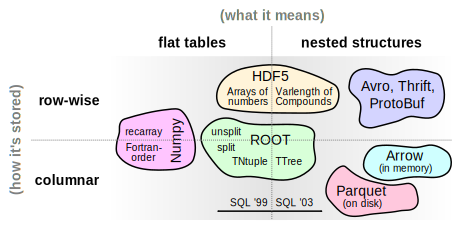
\includegraphics[width=1.2\linewidth]{table-of-formats.pdf}}}\only<2>{\mbox{\hspace{-1 cm}\includegraphics[width=1.2\linewidth]{table-of-formats-2.pdf}}}
\end{frame}

\begin{frame}{Columnar data representation}
\vspace{0.2 cm}
\mbox{\hspace{-0.8 cm}\includegraphics[width=1.2\linewidth]{simd.png}}
\end{frame}

\begin{frame}{Columnar nested data}
\vspace{0.5 cm}

\begin{columns}
\column{0.6\linewidth}
Columnar tables are an old idea
\begin{itemize}
\item Fortran arrays
\item most SQL implementations
\end{itemize}

\vspace{0.5 cm}
Columnar versions of rich data are somewhat newer
\begin{itemize}
\item ROOT in physics, late '90s
\item Google Dremel paper, 2010
\item Apache Parquet: disk format
\item Spark 2.0 memory management
\item Apache Arrow: memory format
\end{itemize}

\column{0.35\linewidth}
\includegraphics[width=\linewidth]{columnar.png}
\end{columns}
\end{frame}

\begin{frame}{Shredding data}
\vspace{0.5 cm}

\mbox{\hspace{-0.25 cm}\begin{minipage}{1.02\linewidth}
Turning a nested data representation into flat arrays is known as ``splitting'' (ROOT), ``striping'' (Dremel), or ``shredding'' (Parquet).

\vspace{0.5 cm}
The data are simply flattened into structureless arrays; structure is encoded in auxiliary arrays (``r'' and ``d'' in this Dremel example).
\end{minipage}}

\vspace{0.5 cm}
\mbox{\hspace{-0.75 cm}\includegraphics[width=1.15\linewidth]{dremel.png}}
\end{frame}

\begin{frame}{Four ways to shred data}
\Large
\begin{itemize}\setlength{\itemsep}{0.5 cm}
\item Recursive counters (my development)
\item Dremel/Parquet style
\item Arrow style
\item Normal form (traditional database theory)
\end{itemize}
\end{frame}

\begin{frame}{But first\ldots\ what types do we need?}
\vspace{0.5 cm}

Type systems can be built in layers, each encoding {\it within} the underlying layer.

\vspace{0.5 cm}
\only<1>{\mbox{\hspace{-0.75 cm}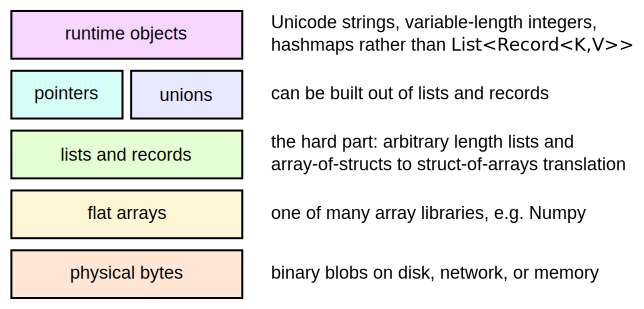
\includegraphics[width=1.15\linewidth]{tower-of-types.pdf}}}\only<2>{\mbox{\hspace{-0.75 cm}\includegraphics[width=1.15\linewidth]{tower-of-types-2.pdf}}}
\end{frame}

\begin{frame}[fragile]{Method \#1: recursive counters}
\vspace{0.5 cm}

Start with a simple idea: flatten arbitrary-length lists into a single array and add a ``counter'' array to specify the length of each list.

\vspace{0.5 cm}
\uncover<2->{The above is limited to one level of depth, so make the counter recursive: it counts the number of elements in a list, then each sublist, then each subsublist, in a single, unbroken stream.}

\vspace{0.5 cm}
\begin{uncoverenv}<3->
{\bf Example:} to encode {\tt\footnotesize List<List<Record<a:integer,b:float>>>}

\scriptsize\bf
\begin{Verbatim}[commandchars=\\\{\}]
value   \textcolor{blue}{[} \textcolor{violet}{[}(\textcolor{red}{1}, \textcolor{darkgreen}{1.1})\textcolor{violet}{]}, \textcolor{violet}{[]}, \textcolor{violet}{[}(\textcolor{red}{2}, \textcolor{darkgreen}{2.2}), (\textcolor{red}{3}, \textcolor{darkgreen}{3.3})\textcolor{violet}{]} \textcolor{blue}{]}, \textcolor{blue}{[} \textcolor{violet}{[}(\textcolor{red}{4}, \textcolor{darkgreen}{4.4})\textcolor{violet}{]} \textcolor{blue}{]}

counter \textcolor{blue}{3},\textcolor{violet}{1},          \textcolor{violet}{0},  \textcolor{violet}{2},                      \textcolor{blue}{1},\textcolor{violet}{1}
data-a      \textcolor{red}{1},              \textcolor{red}{2},        \textcolor{red}{3},              \textcolor{red}{4}
data-b         \textcolor{darkgreen}{1.1},            \textcolor{darkgreen}{2.2},      \textcolor{darkgreen}{3.3},            \textcolor{darkgreen}{4.4}
\end{Verbatim}
\end{uncoverenv}

\vspace{0.3 cm}
\uncover<4->{Lossless encoding: original list-of-lists can be recovered by walking over counter with a stack of indexes.}
\end{frame}

\begin{frame}{Method \#2: Dremel/Parquet style}
\vspace{0.25 cm}
\begin{center}
\only<1>{\includegraphics[width=0.88\linewidth]{repetition-levels-2.png}}\only<2>{\includegraphics[width=0.88\linewidth]{repetition-levels.png}}\only<3>{\includegraphics[width=0.8\linewidth]{definition-levels-2.png}}\only<4>{\includegraphics[width=\linewidth]{definition-levels.png}}
\end{center}
\end{frame}

\begin{frame}[fragile]{Method \#2: Dremel/Parquet style}
\vspace{0.5 cm}
Definition levels aren't optional: you can't encode empty lists without them.

\vspace{0.5 cm}
{\bf Example:} to encode {\tt\footnotesize List<List<Record<a:integer,b:float>>>}

\scriptsize\bf
\begin{Verbatim}[commandchars=\\\{\}]
value   \textcolor{blue}{[} \textcolor{violet}{[}(\textcolor{red}{1}, \textcolor{darkgreen}{1.1})\textcolor{violet}{]}, \textcolor{violet}{[]}, \textcolor{violet}{[}(\textcolor{red}{2}, \textcolor{darkgreen}{2.2}), (\textcolor{red}{3}, \textcolor{darkgreen}{3.3})\textcolor{violet}{]} \textcolor{blue}{]}, \textcolor{blue}{[} \textcolor{violet}{[}(\textcolor{red}{4}, \textcolor{darkgreen}{4.4})\textcolor{violet}{]} \textcolor{blue}{]}

replevel    0,        \fbox{1,}\,\,  1,        2,              0
deflevel    2,        \fbox{1,}\,\,  2,        2,              2
data-a      \textcolor{red}{1},              \textcolor{red}{2},        \textcolor{red}{3},              \textcolor{red}{4}
data-b         \textcolor{darkgreen}{1.1},            \textcolor{darkgreen}{2.2},      \textcolor{darkgreen}{3.3},            \textcolor{darkgreen}{4.4}
\end{Verbatim}

\normalsize\sf
\vspace{0.3 cm}
\begin{uncoverenv}<2->
Dremel/Parquet style packs tightly without compression, but it's unclear how relevant that is with fast compression (e.g.\ snappy).

\vspace{0.25 cm}
It also adds a lot of complexity; unclear how to present this data as an iterator.
\end{uncoverenv}
\end{frame}




\end{document}
